\chapter{数据同步与平滑机制的引入}
\section{初步运行测试}
经过第四章中设计与实现的内容后,我们得到了一个可以连接仿真机和图像生成器并转换双方指令的数据交换子系统。
为测试系统在真实FFS环境下的表现,需要去到飞行训练基地接入专业设备进行初步的功能测试。
\subsection{测试环境}
为使用真实仿真机设备,我们去到南方航空珠海训练基地。此处是亚洲最大,机型最全的模拟飞行训练基地,共拥有28台民航局运输司认证的最高D等级FFS,每年有超过7000名飞行员在此训练,是名副其实的中国民航飞行员培养摇篮。
\par
该测试环境中各设备布置方式如图\ref{testenv}所示。虚拟仿真机需要配置两张网卡,一张通过交换机连接仿真机,另一张通过交换机连接三台图像生成器。
三台图像生成器各自连接一台投影仪才能实现对模拟座舱前方球幕的融合投影。
\begin{figure}[h!]
    \begin{center}
        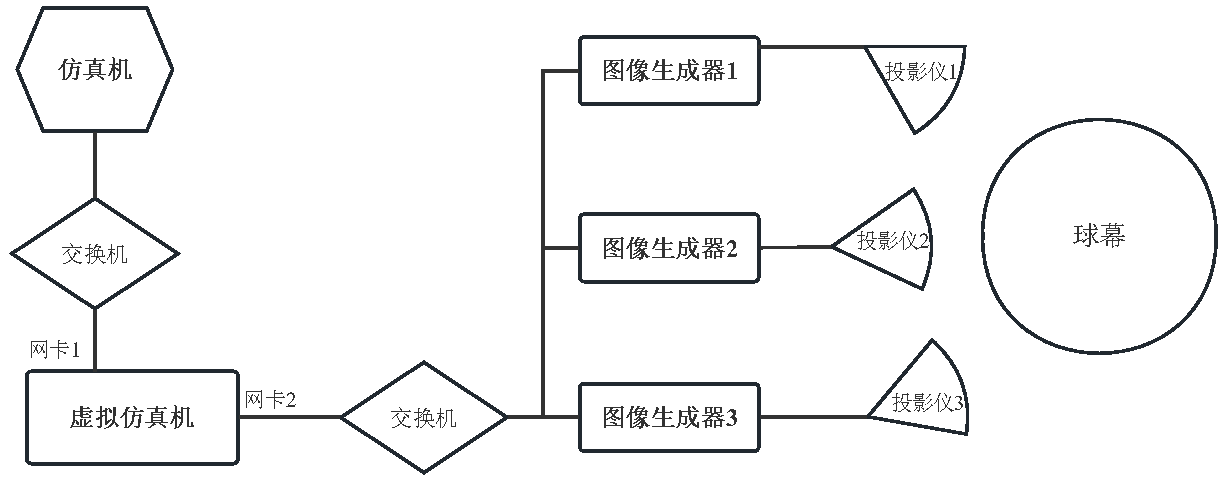
\includegraphics[width=\textwidth]{pictures/testenv.pdf}
        \caption{测试环境设备布置}
        \label{testenv}
    \end{center}
\end{figure}
\par
此环境下虚拟仿真机运行于一台机器上,三台图像生成器运行在配置完全相同的三台机器上,它们通过网线连接交换机。
为了顺利运行视景系统,运行设备上需要配置系统运行的软件环境,详细信息如表\ref{devsoft}所示。
虚拟仿真机和图像生成器两方都需要C++与Python的运行环境,且双方需要通过Tbuspp插件沟通。
在虚拟仿真机中,需要使用WinPcap软件侦听流经网卡的数据包。测试环境部署配置完成后应当能保证系统不会因为软件环境问题无法运行。

\begin{table}[h!]
    \begin{center}
        \caption{软件配置表}
        \label{devsoft}
        \renewcommand\arraystretch{1.5}
        \begin{tabularx}{0.8\textwidth}{ 
             >{\centering\arraybackslash\hsize=.5\hsize\linewidth=\hsize}X 
             >{\centering\arraybackslash\hsize=\hsize\linewidth=\hsize}X 
             }
             \hline
            \textbf{配置项 } & \textbf{详情}\\
             \hline
             C++运行环境 & VS\_C++\_MSVC\\
           
             Python运行环境 & Python\thinspace 3.10\\
             
             底层网络访问 & WinpCap\thinspace v4.1.3\\
            
             服务网格 & Tbuspp \thinspace 0.6.0\\
             \hline
            \end{tabularx}
    \end{center}
\end{table}
\par
在硬件配置方面,运行图像生成器的机器基本配备最新且性能最强的配件,保障渲染帧率能跟上仿真机产生数据的频率。测试环境下的具体硬件配置信息如表\ref{ffshard}所示。
测试环境中的网络完全隔绝外部网络,网络环境非常良好,网络时延在1ms内,网络抖动几乎为0。也意味着如果测试中出现问题,网络环境并不是一个首先需要考虑的因素。

\subsection{功能测试}
对于本数据交换子系统的功能测试依照指令代号进行。第三章中提到目前已经验证了21种仿真机指令,我们让飞行员和教练员在模拟座舱中进行操作依次产生这些指令,
如果投影画面产生了对应指令代号的变化,则说明数据交换子系统对于该类指令的接收、转换、发送、分配使用的过程顺利,可以通过测试。
表\ref{testcase}给出了对于仿真机指令代号为21H指令的测试用例,该指令负责控制飞机的位置和姿态,其他种类指令的测试用例与此表类似。
\clearpage
\begin{table}[h!]
    \begin{center}
        \caption{硬件配置表}
        \label{ffshard}
        \renewcommand\arraystretch{1.5}
        \begin{tabularx}{\textwidth}{ 
             >{\centering\arraybackslash\hsize=.4\hsize\linewidth=\hsize}X 
             >{\centering\arraybackslash\hsize=.4\hsize\linewidth=\hsize}X 
             >{\centering\arraybackslash\hsize=\hsize\linewidth=\hsize}X 
             }
             \hline
            \textbf{设备} & \textbf{配置项} & \textbf{详情}\\         
             \hline
             & CPU & Intel® Core™ i9-12900K Processor\\
           
             & GPU & NVIDIA RTX A6000\\
             
             图像生成器 & 内存 & 64GB\\
            
             & 硬盘 & 8TB\\
             
             & 系统 & Windows 10 专业版 21H2\\
             \hline
             & CPU & Intel® Core™ i9-12900K Processor\\
           
             & GPU & Intel® UHD Graphics 770\\
             
             虚拟仿真机 & 内存 & 32GB\\
            
             & 硬盘 & 2TB\\
             
             & 系统 & Windows 10 专业版 21H2\\
             \hline
             
            \end{tabularx}
    \end{center}
\end{table}
\begin{table}[h!]
    \begin{center}
        \caption{控制指令21H测试用例}
        \label{testcase}
        \renewcommand\arraystretch{1.5}
        \begin{tabularx}{0.8\textwidth}{ 
             >{\centering\arraybackslash\hsize=.2\hsize\linewidth=\hsize}X 
             >{\raggedright\arraybackslash\hsize=.8\hsize\linewidth=\hsize}X 
             }
             \hline
            \textbf{ID } & \textbf{TC1}\\
             \hline
             \textbf{测试名称} & 仿真机21H指令控制测试\\
             \hline
             \textbf{待测功能} & 图像生成器能接收并使用转换后的21H指令。\\
             \hline
             \textbf{测试步骤} & 1.飞行员通过操纵杆让飞机运动。\par 2.仿真机生成21H指令。\par 3.虚拟仿真机转换其为自定义指令。\par 4.图像生成器收到指令分配给对应处理逻辑。  \\
             \hline
             \textbf{预期结果} & 投影画面中的飞机按飞行员的操作运动。\\
             \hline
            \end{tabularx}
    \end{center}
\end{table}
\par
图\ref{21test}展示了投影画面中的飞机根据飞行控制指令沿跑道起飞的过程。证明数据交换子系统对该指令的处理流程通过测试。

\par
图\ref{todtest}展示了投影画面对时间变换指令的响应效果。模拟场景中精确到一天中的每一分钟都可以由时间变换指令控制,
图中是将时间调整到黄昏时分的环境效果。指令被正确应用,数据交换子系统对时间变换指令的处理流程通过测试。
\clearpage
\begin{figure}[h!]
    \begin{center}
        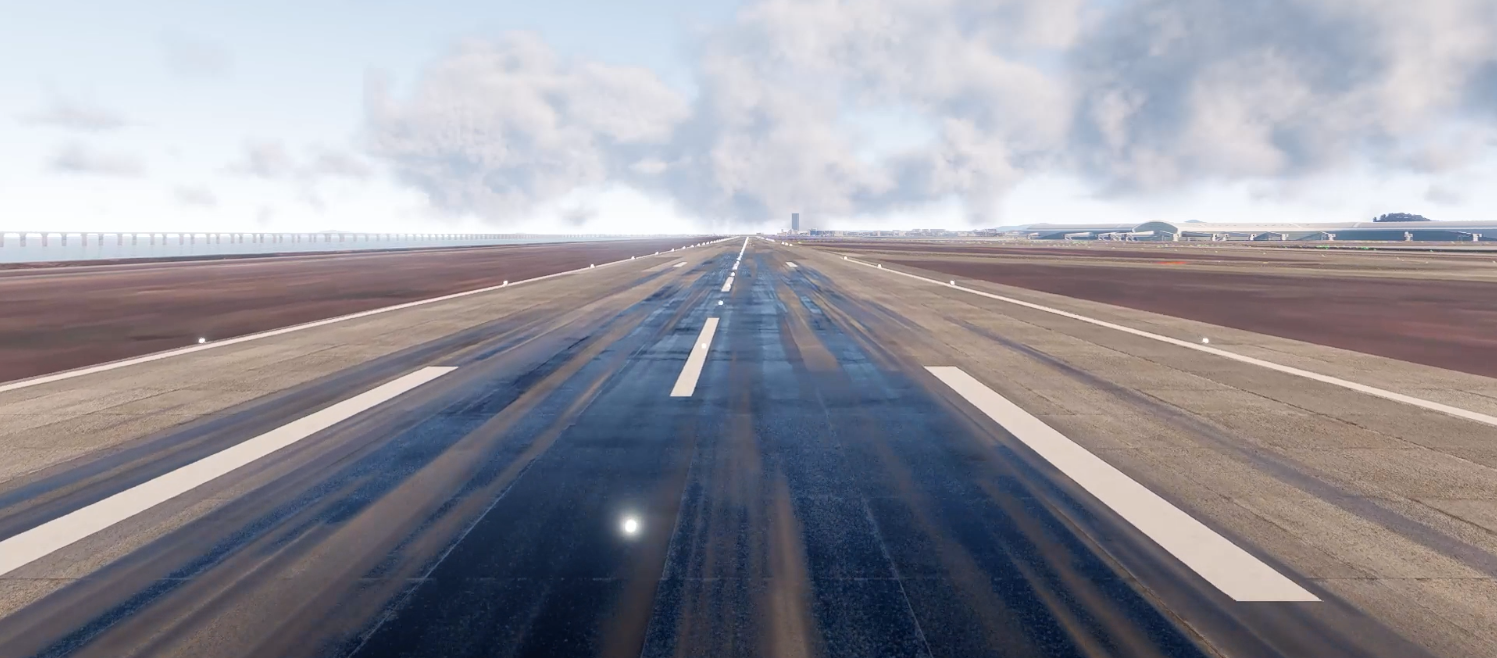
\includegraphics[width=.9\textwidth]{pictures/firstcamera.png}
        \caption{飞行控制指令测试结果}
        \label{21test}
    \end{center}
\end{figure}
\begin{figure}[h!]
    \begin{center}
        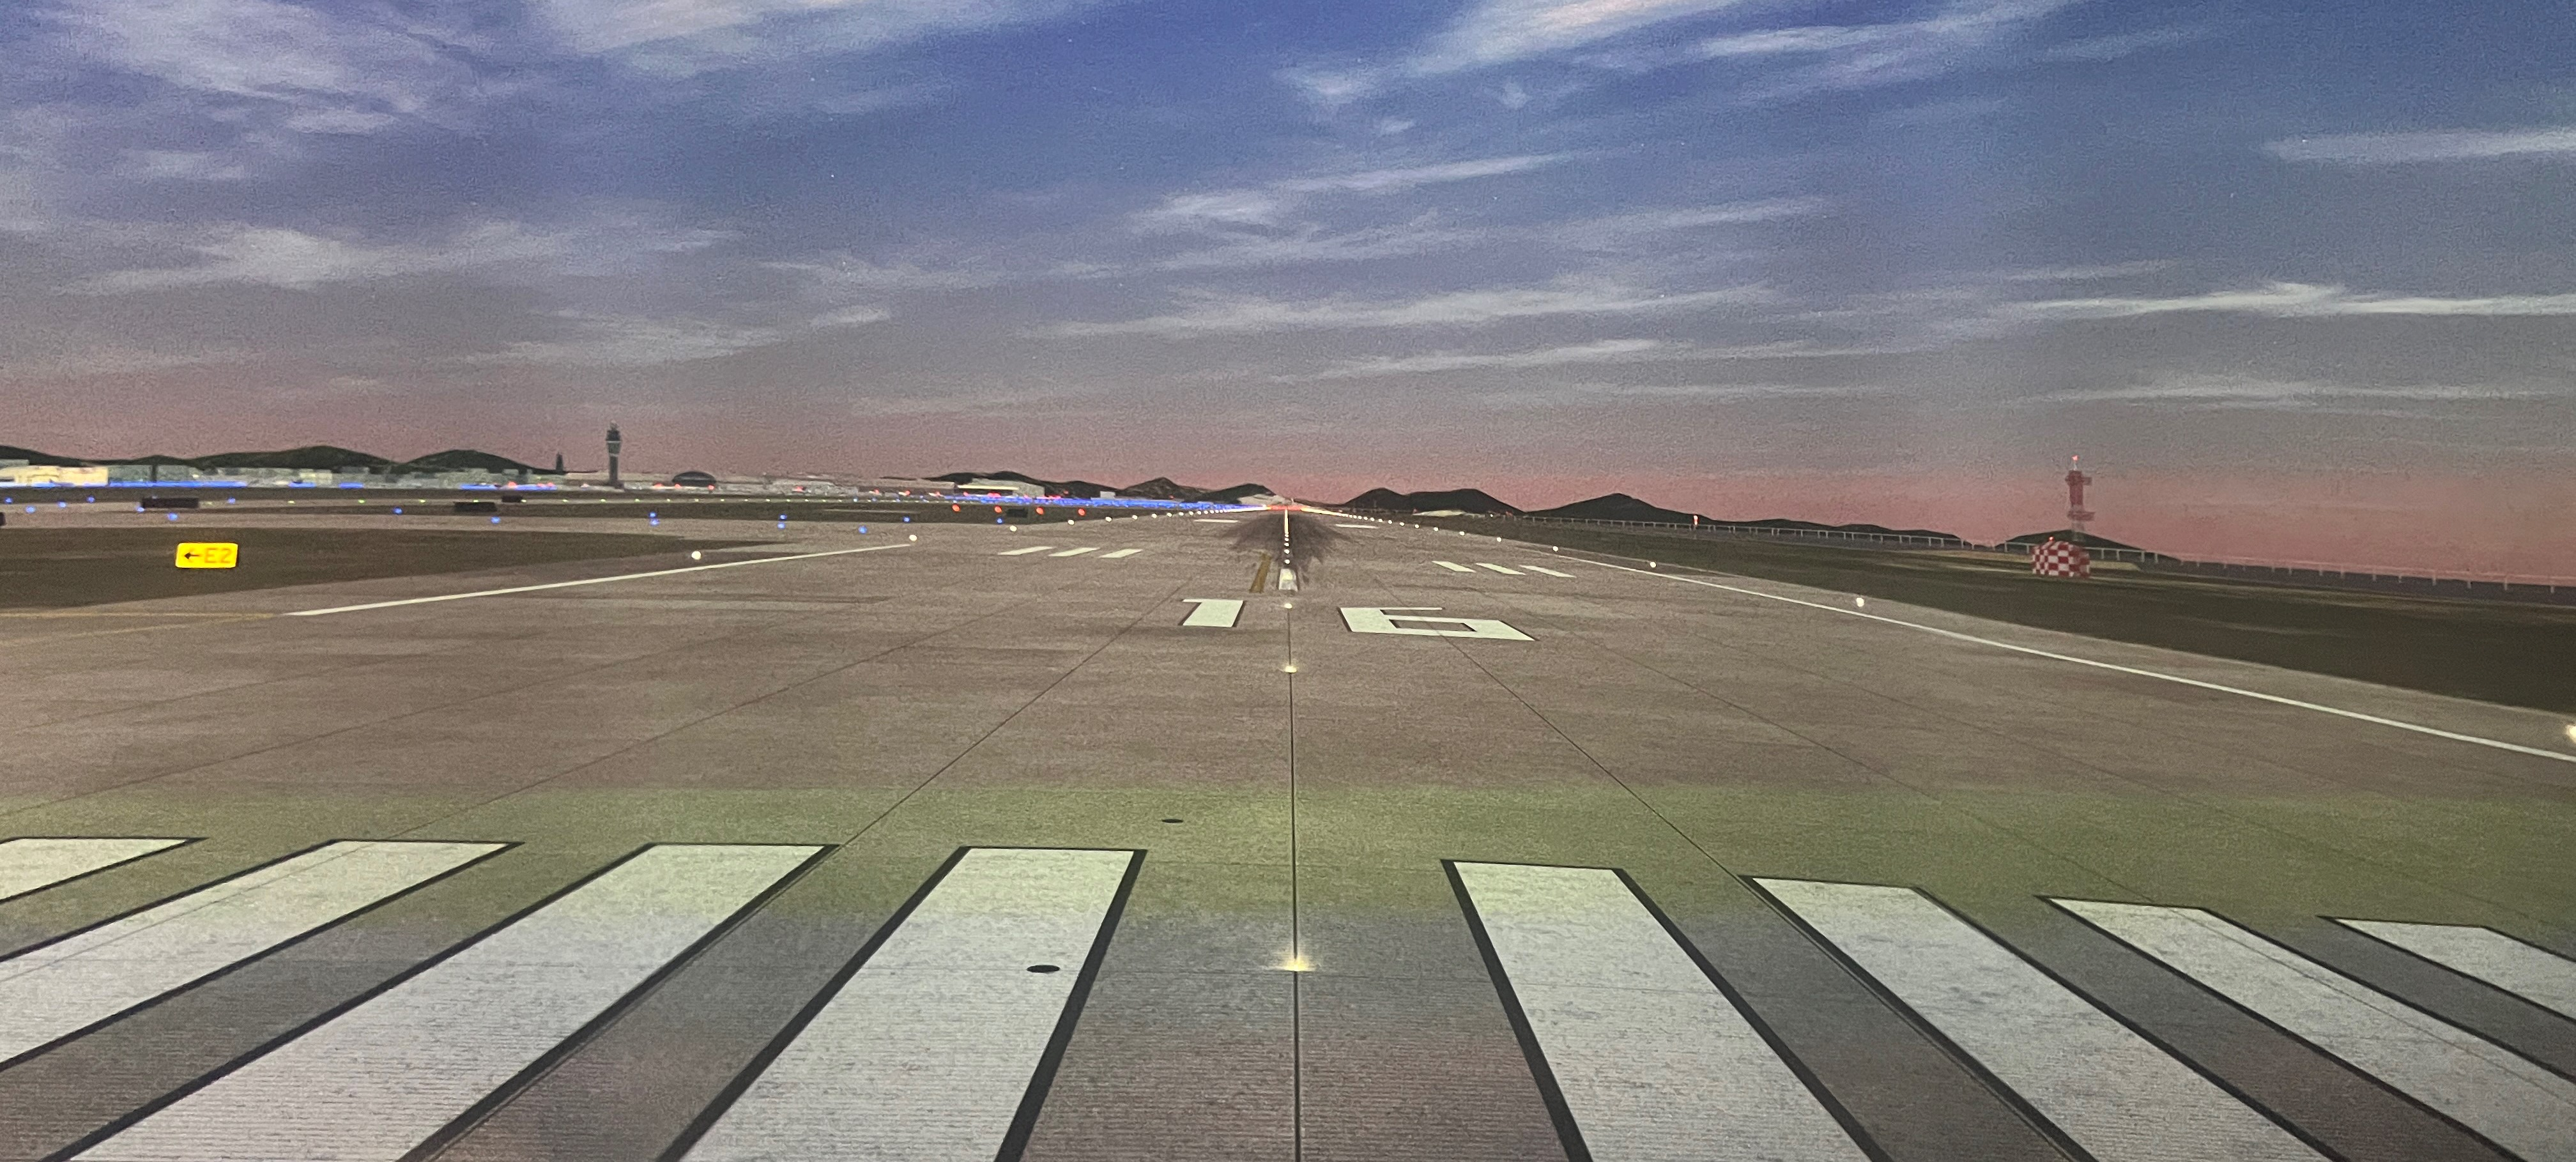
\includegraphics[width=.9\textwidth]{pictures/todtest.jpg}
        \caption{时间变换指令测试结果}
        \label{todtest}
    \end{center}
\end{figure}
\par
图\ref{lighttest}展示了投影画面对灯光控制指令的响应效果。飞机身上诸如滑行灯、机翼灯、防撞灯等多种灯光的开关控制均由灯光指令控制。
图中是飞机在夜间开启滑行灯后的视景效果。指令可以正确应用,数据交换子系统对灯光指令的处理流程通过测试。
\par
图\ref{snowtest}展示了投影画面对天气控制指令的响应效果。飞行过程中的雨雪天气及等级都由天气指令控制,图中展示了视景中大雪天气的效果,
视野中不仅有雪花的加入,能见度也大大降低。指令被正确应用,数据交换子系统对天气指令的处理流程通过测试。
\clearpage
\begin{figure}[h!]
    \begin{center}
        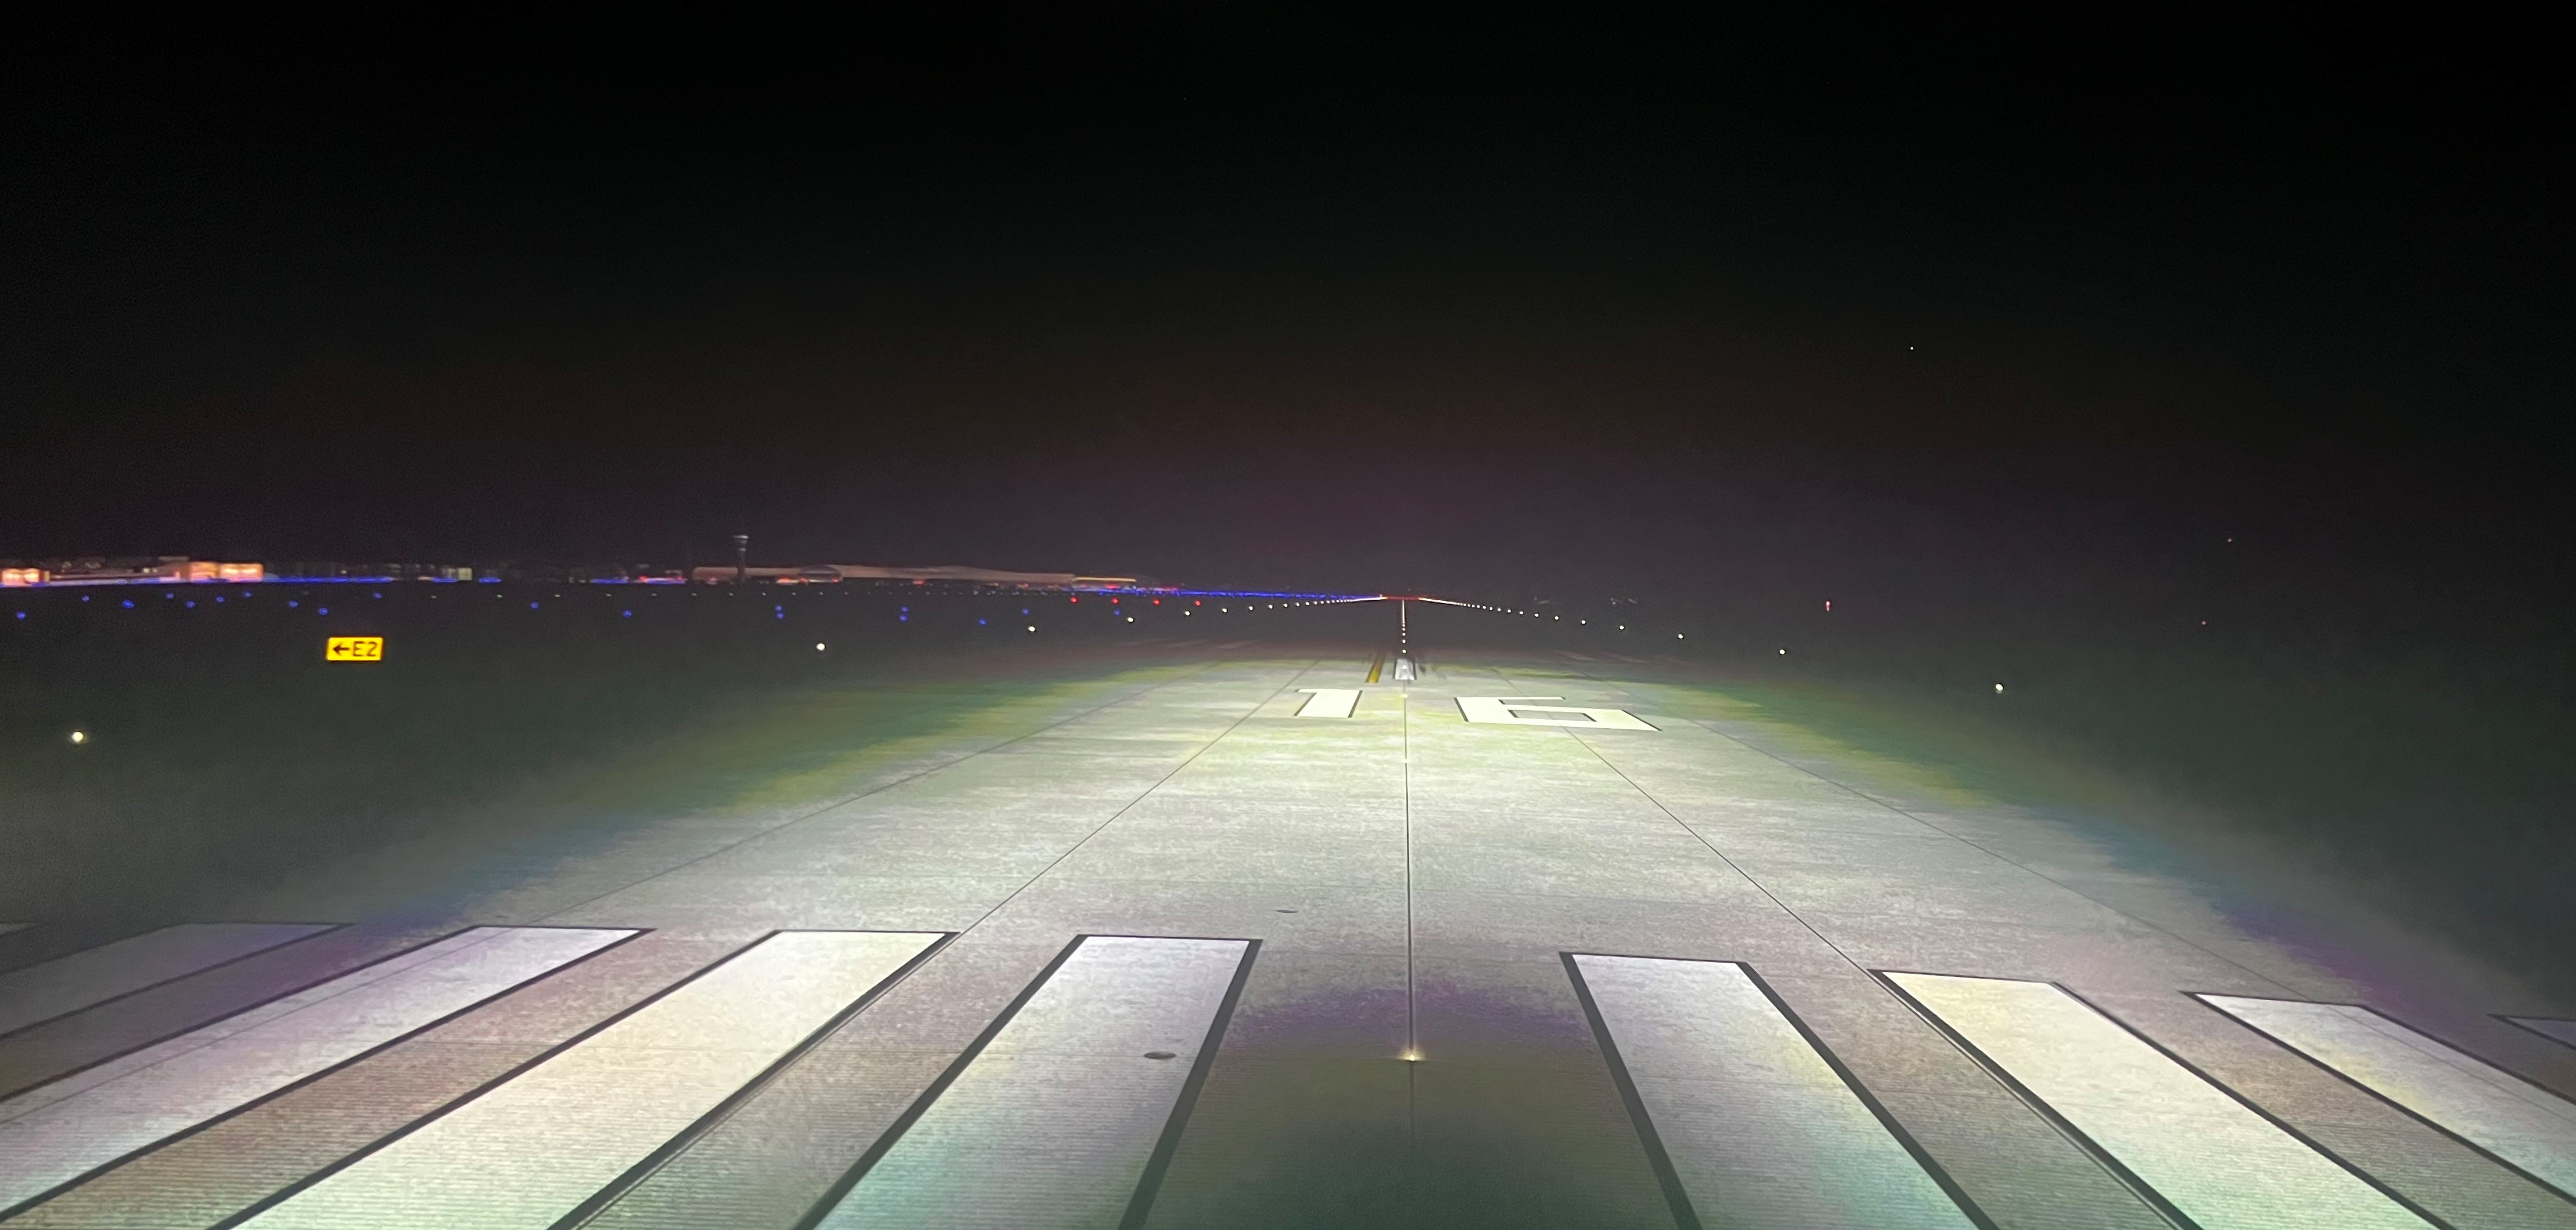
\includegraphics[width=.9\textwidth]{pictures/lighttest.jpg}
        \caption{灯光指令测试结果}
        \label{lighttest}
    \end{center}
\end{figure}
\begin{figure}[h!]
    \begin{center}
        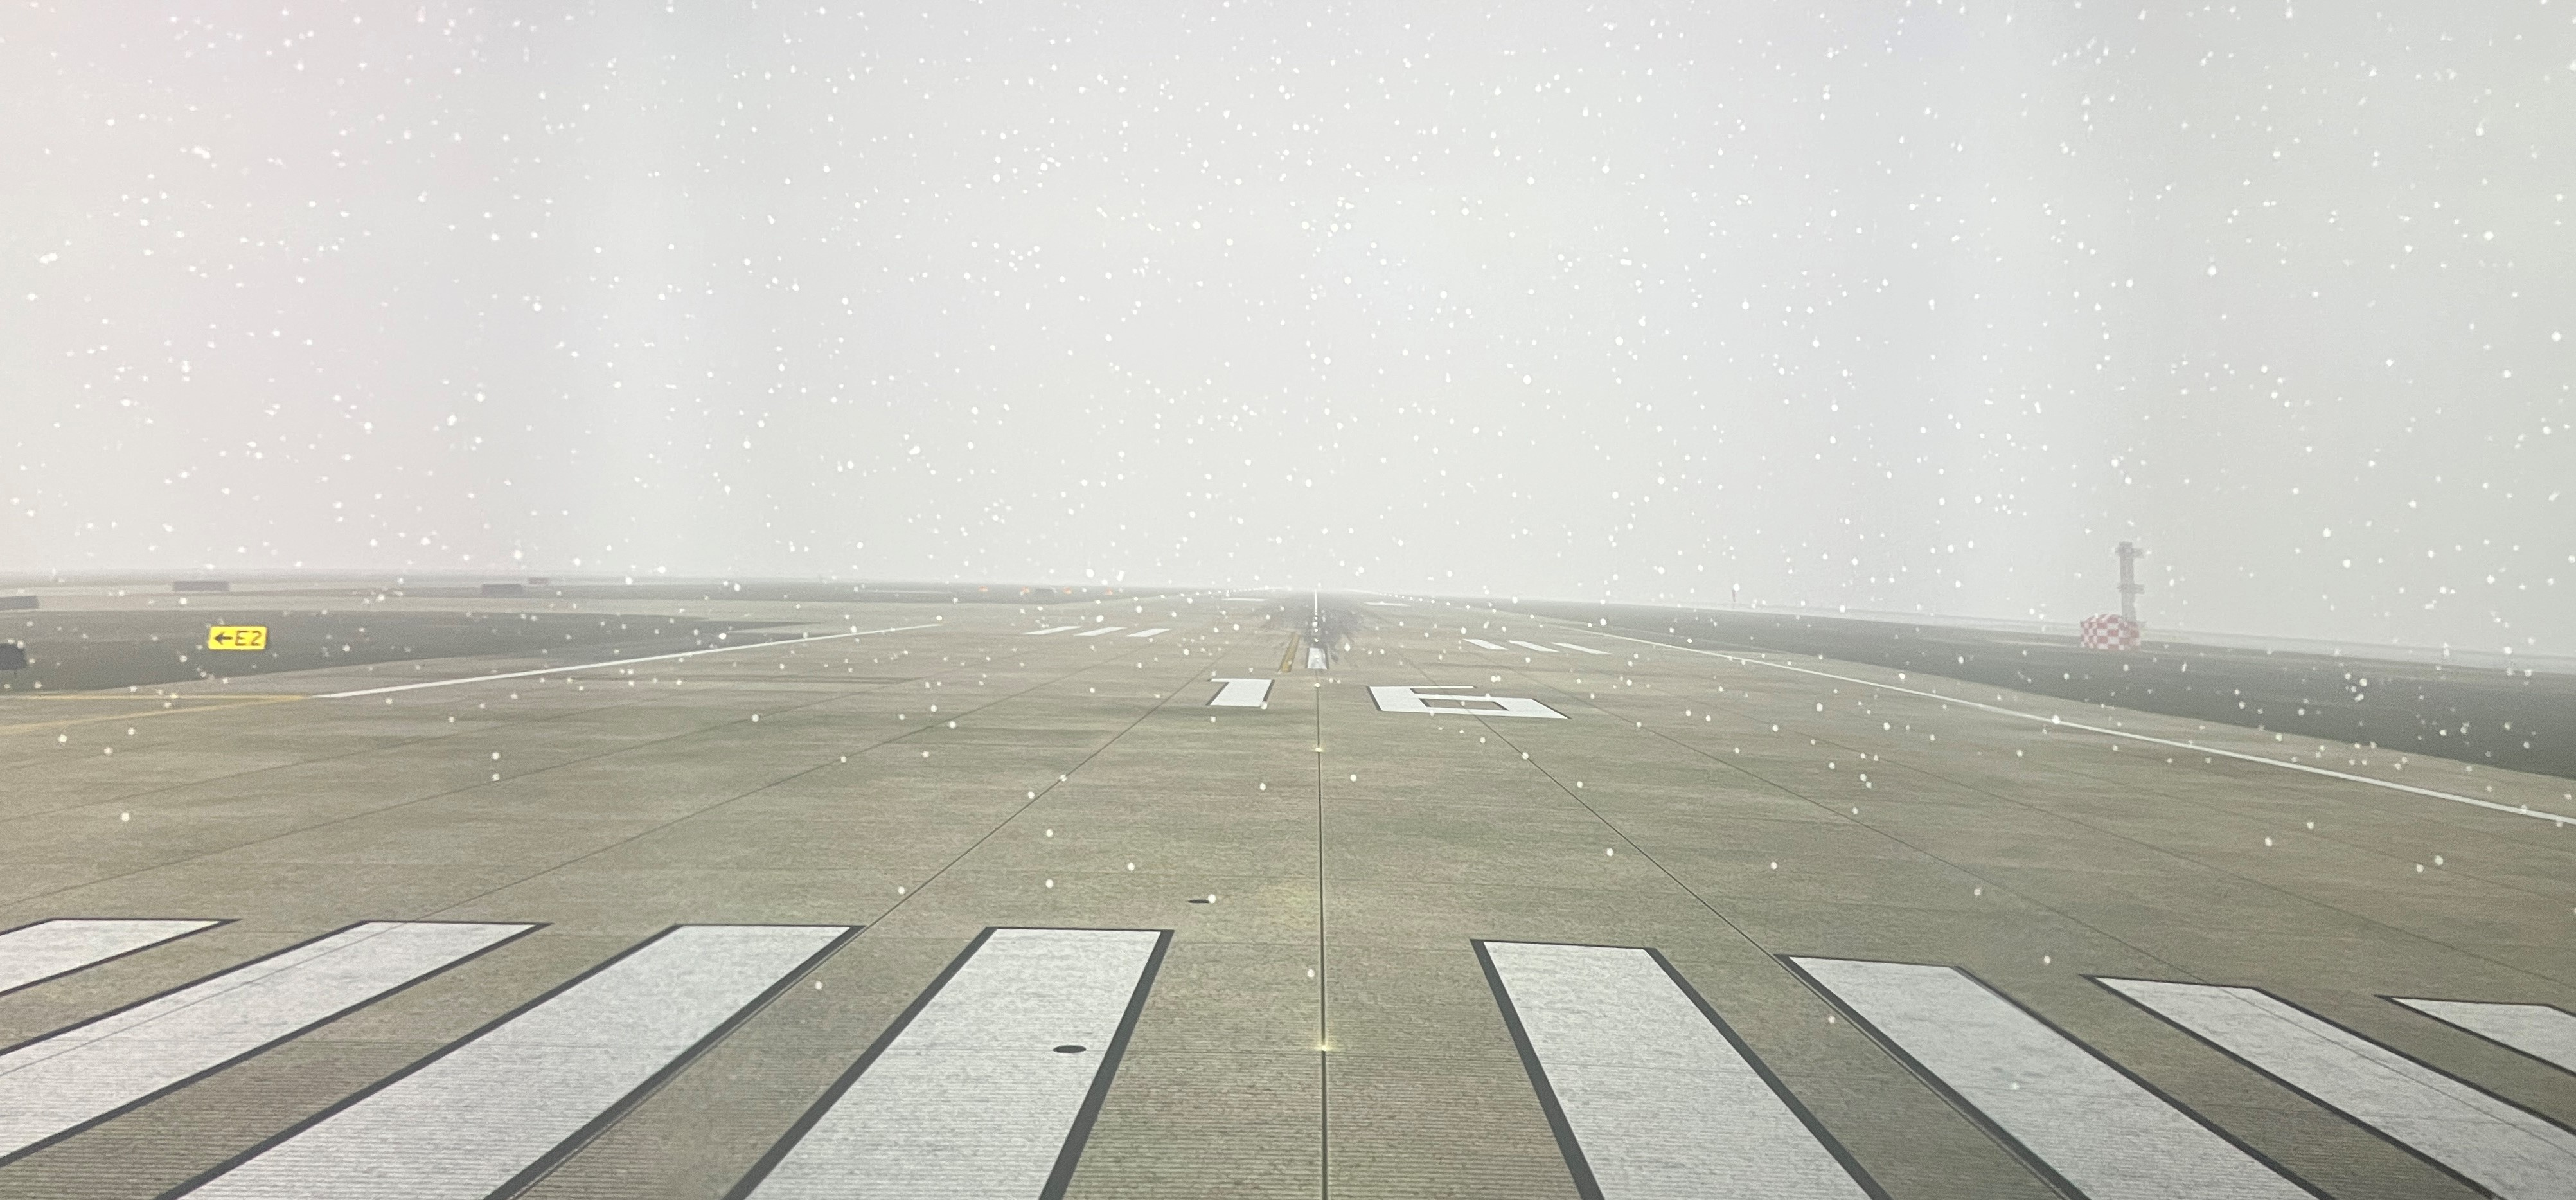
\includegraphics[width=.9\textwidth]{pictures/snowtest.jpg}
        \caption{天气指令测试结果}
        \label{snowtest}
    \end{center}
\end{figure}
\par
当然已通过验证的仿真机指令远不止这些,此处不再逐一列举测试情况。
飞行过程中会产生一些需送回仿真机的反馈指令,比如飞机在起飞和降落过程中会持续检测三个起落架的离地高度。
测试时我们对比了图像生成器构建的自定义指令与从仿真机侧捕获到的仿真机指令中的内容。
表\ref{fbcomp}展示了两方数据的对比结果,仿真机对于高度使用的单位是0.5mm,经换算后与自定义指令一致。
说明数据交换子系统可以正确处理该反馈指令。
\begin{table}[h!]
    \begin{center}
        \caption{反馈信息对比}
        \label{fbcomp}
        \renewcommand\arraystretch{1.5}
        \begin{tabularx}{0.8\textwidth}{ 
             |>{\centering\arraybackslash\hsize=.7\hsize\linewidth=\hsize}X 
             |>{\centering\arraybackslash\hsize=1.15\hsize\linewidth=\hsize}X 
             |>{\centering\arraybackslash\hsize=1.15\hsize\linewidth=\hsize}X
             |
             }
             \hline 
            \textbf{起落架编号} & \textbf{自定义指令} & \textbf{仿真机指令}\\   
             \hline
             1 & 3.822m & 7644\\
             \hline
             2 & 3.787m & 7574\\     
             \hline
             3 & 3.787m & 7574\\
             \hline 
             ...& ... & ...\\
             \hline 
             1 & 40.031m & 80062\\
             \hline 
             2 & 39.914m & 79828\\
             \hline 
             3 & 39.912m & 79824\\
             \hline  
            \end{tabularx}
    \end{center}
\end{table}

\section{数据同步机制}
\subsection{问题分析}
本次测试中同样发现了一些问题。
最具代表性的问题如图\ref{tear}红框中所示,发现在飞行的过程中融合投影的图像中存在撕裂现象。
此处说的图像撕裂并非传统的同一个显示设备的图像上下两部分的撕裂,因为采用了投影仪垂直同步也不会产生这种撕裂。
此时的撕裂是在两台投影仪的交界处存在左右两部分撕裂,即两台设备各自渲染的部分图像并不能完美拼接在一起。
且就整体画面而言,偶尔会出现肉眼可观察的顿挫现象,即存在跳帧的问题。
\begin{figure}[h!]
    \begin{center}
        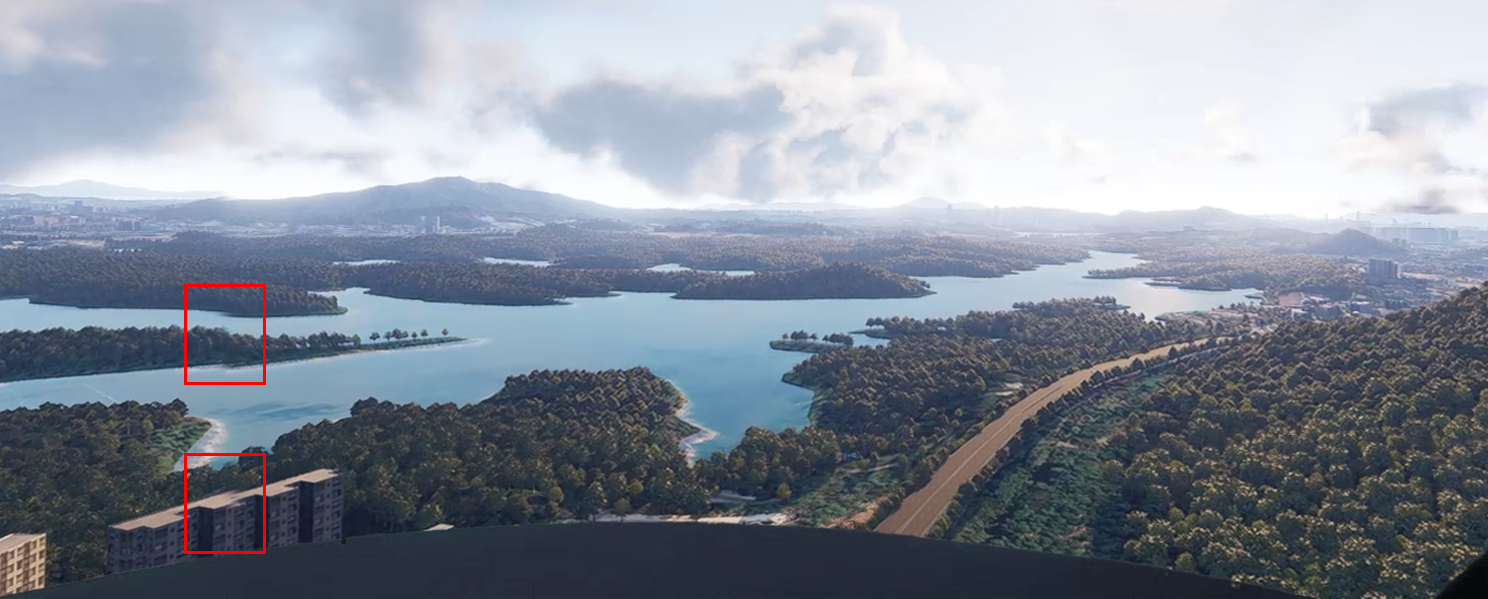
\includegraphics[width=\textwidth]{pictures/tearmark.png}
        \caption{画面撕裂情况}
        \label{tear}
    \end{center}
\end{figure}
\par
对于此现象首先考虑是否投影图像本身就无法拼接,即投影仪校准或多台图像生成器各自渲染时的投影矩阵存在问题,但比较明确的是在飞机静止时并不会出现如上的画面撕裂问题,
这证明并非图像本身无法拼接。由此便仅有一种可能性,便是多台投影仪的投影图像并非同一帧的内容,两侧的图像间产生了差距所以不能拼接。
图\ref{tearreason}展示了投影帧不能及时更新的原因。图像生成器的逻辑帧需要收到投影仪V-Sync信号后才能执行,但在本场景中逻辑帧的执行要依赖于从仿真机发送来的指令内容,
如果此时指令并未送达便会错过这一更新周期,导致投影图像不会改变。如果其他的图像生成器即时获得了指令,则会正常更新图像,便会领先一帧的内容,产生图像撕裂。
\par
如果一台图像生成器多次错过更新周期则会导致跳帧,即缓存中的某些帧未经投影直接被覆盖,产生视觉上的顿挫感。
\begin{figure}[h!]
    \begin{center}
        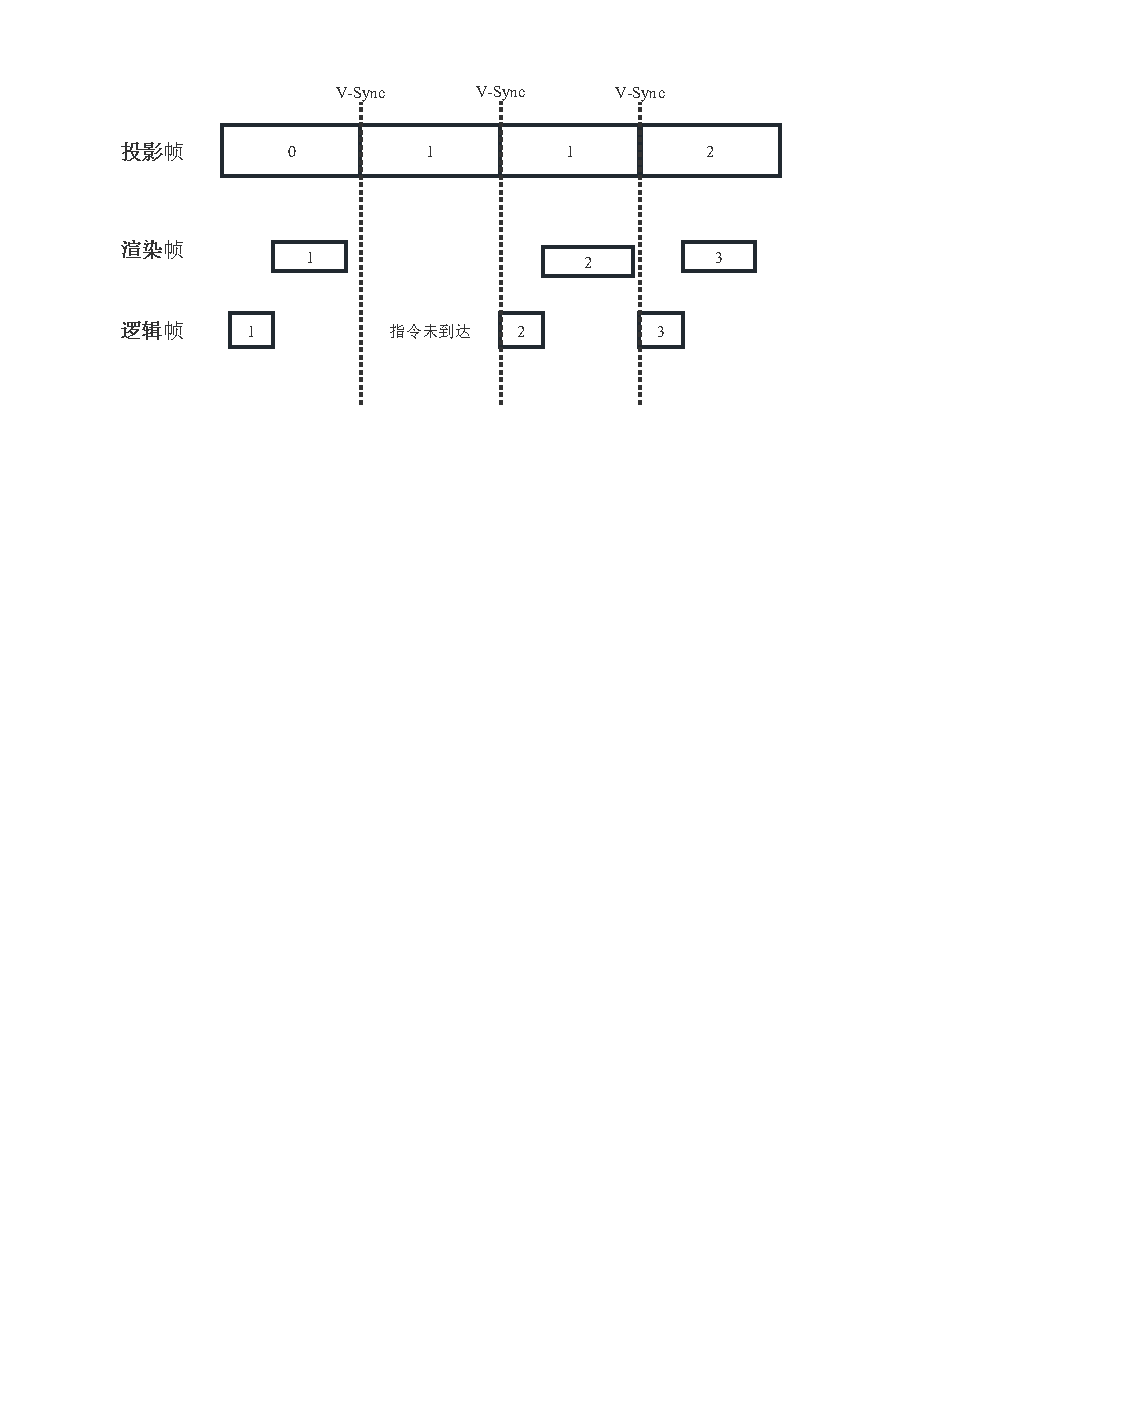
\includegraphics[width=\textwidth]{pictures/tearreason.pdf}
        \caption{更新周期的丢失}
        \label{tearreason}
    \end{center}
\end{figure}
\par 
接下来就需要排查指令不能及时到达图像生成器的原因。前面提到机房的网络环境十分优秀,网络波动基本可以排除。
结合整个指令流动过程,可能使指令到达频率不稳定的地方有二,一是发送给多台图像生成器时存在时间上的差距,二是虚拟仿真机接收仿真机指令的频率不稳定。
其中,第一点的原因比较明确,因为虚拟仿真机与图像生成器间采用TCP通信,TCP不持支广播所以无法同时向多个图像生成器发送相同的指令数据。
轮询发送的结果是最后一台机器收到数据的时间大约慢5毫秒,对于60Hz的刷新率来讲该延迟已占据一帧中三分之一的时间,极有可能令某些图像生成器错过更新周期。
\par
对于第二点的检查则监控了虚拟仿真机接收数据帧的时刻,图\ref{}展示了记录的日志结果。从中发现在仿真机以标准60Hz的频率产生数据帧的情况下,即使WinPcap开启了立即转发模式,
虚拟仿真机每分钟也会产生约10次3毫秒的接收延迟。当然这个延迟对于多台图像生成器而言是统一的,可能会同时错过这一帧的更新,产生顿挫。
% TODO:log日志文件
\subsection{网络帧缓冲}
从以上分析可知,造成问题的原因是在图像生成器需要使用指令数据时,接收队列中可能并没有准备好的数据供使用。
如果在图像生成器侧准备一个对于指令的缓冲,当队列中的指令达到一定数目时再开始运转,就可以有效缓解这些问题。
当然引入缓冲机制后一定会造成操作响应上的延迟,根据官方标准来讲,真实的飞机响应飞行员的操作本就存在延迟,模拟飞行中,要求视景系统可以在这个延迟的基础上在120毫秒内产生响应。
而在60Hz工作频率下,我们对指令的转换,缓冲加渲染的时间相较而言绰绰有余,增加几帧的缓冲并不影响达到标准。
\par
如图\ref{framebuffer}所示,如果网络帧缓冲的数值被设为2,那么图像生成器需要等待当前频率下第三个周期的时刻再开始执行第一帧逻辑。
此时的指令队列中一定已存在两个以上的指令内容,此时再使用指令1去执行第一帧的逻辑就不会出现指令未到达而错过更新周期的问题。
此方法可以同时屏蔽来自TCP逐个发送的时间差和虚拟仿真机接收仿真机指令时的频率不稳定。
\begin{figure}[h!]
    \begin{center}
        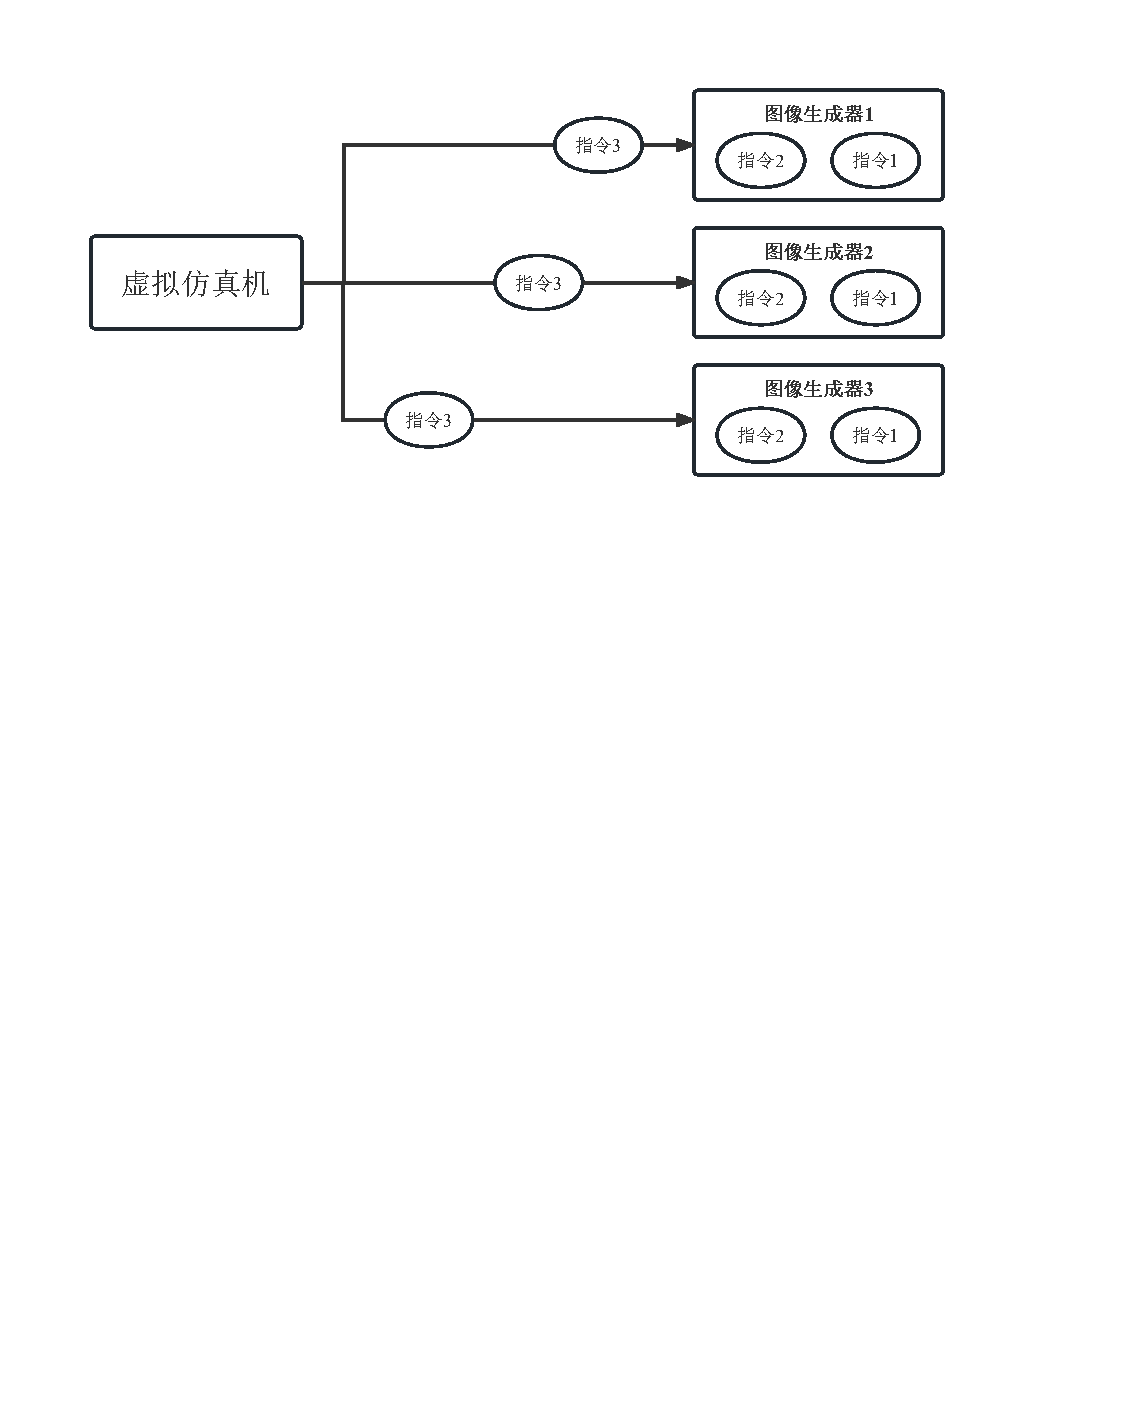
\includegraphics[width=\textwidth]{pictures/framebuffer.pdf}
        \caption{网络帧缓冲示意图}
        \label{framebuffer}
    \end{center}
\end{figure}
\par
图\ref{framebuf}是网络帧缓冲机制的关键代码,Tbuspp中接收到的通用结构packet会被加入circue\_queue\_队列中,
该结构的头部含有数据发送方信息source,我们首先按照发送方将该通用结构分开存放到received\_packets\_中。
之后需要读取Tbuspp相关设置中的帧缓冲信息cachedFrameCount以决定使用几帧网络帧缓冲。
随后便需要对received\_packets\_中的指令数据进行处理,目前我们仅处理发送方为仿真机的数据。如果该发送方对应的帧缓存数量还没有超过设定值,那么便不能交由逻辑处理,
继续等待更多指令的到来。超过阈值则可以交给对应的handler去做处理,并将其从缓冲中擦除。
\begin{figure}[h!]
    \centering
     \lstinputlisting[basicstyle= \zihao{-5}]{pictures/framebuf.txt}
    \caption{网络帧缓冲机制代码}
    \label{framebuf}
\end{figure}
\section{数据平滑机制}
\subsection{问题分析}
加入数据帧缓冲机制后,图像撕裂和顿挫现象基本消失,三台图像生成器可以及时获得指令数据并最终完成投影,
但同时又发现在飞机高速运动的时,图像的拼接部分出现了持续的抖动现象。
图\ref{jitter}对该现象做了示意,在图像交界处会在运动方向产生波纹状的持续抖动,在大屏幕上尤其明显。
\begin{figure}[h!]
    \begin{center}
        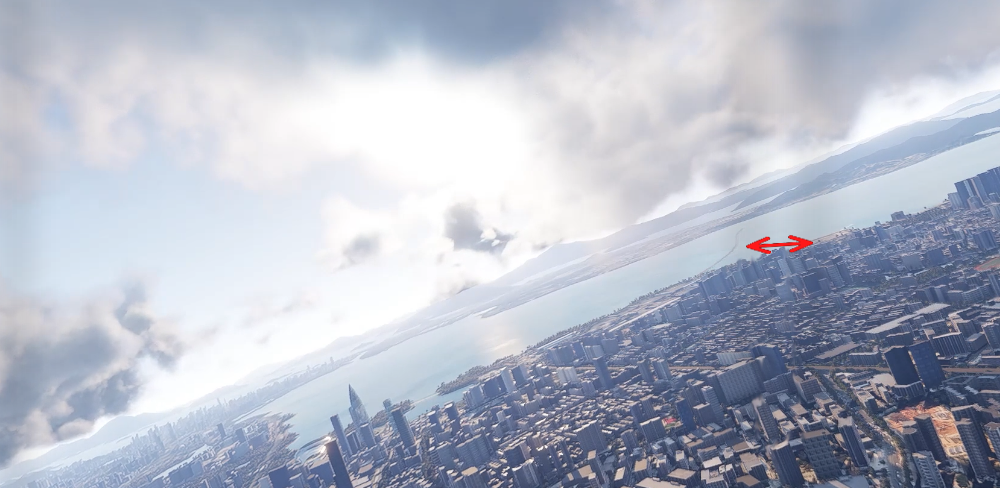
\includegraphics[width=\textwidth]{pictures/jitter.png}
        \caption{画面抖动示意}
        \label{jitter}
    \end{center}
\end{figure}
\par
在引入了帧缓冲机制后,多台投影仪一定会投影同一帧的画面,理论上应该不会再有拼接部分的问题。但是之前忽略了一个问题,虽然多台投影仪拥有相同的刷新率,但是它们每一帧开始的时间可能并不相同。
即如图\ref{present}所示,由于投影仪的刷新时间不同步,会最终影响逻辑帧的开始时间不同。相较于之前图像的撕裂,此问题会导致在一帧以内时间的图像不一致性,且会连续在一致与不一致的状态间转换,由此产生视觉上的抖动效果。
其实此问题也会加剧上一节中提及的图像撕裂问题,在加入帧缓冲后以抖动的形式出现。
\begin{figure}[h!]
    \begin{center}
        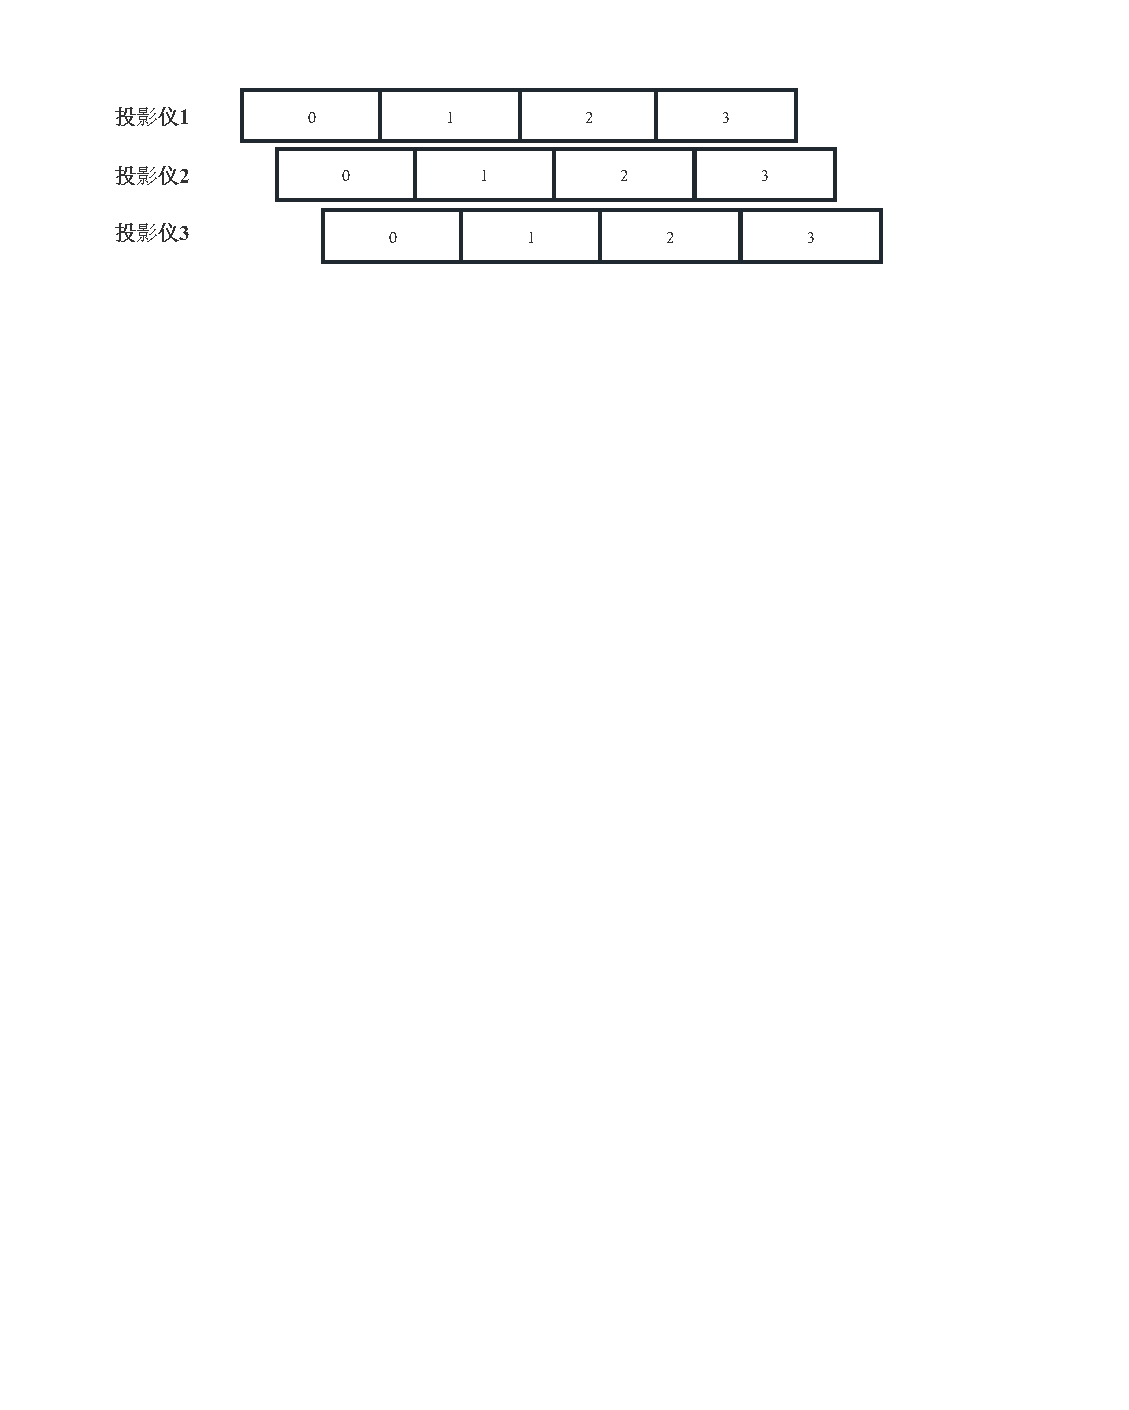
\includegraphics[width=\textwidth]{pictures/present.pdf}
        \caption{多投影仪不同步}
        \label{present}
    \end{center}
\end{figure}
\subsection{插值平滑}
想令多台投影仪同步其实有硬件层面的解决方法,但是需要定制显卡并将多张显卡用专用同步线进行连接,市面上流通的显卡设备并不支持此项功能。
此解决方案的购买成本和后期维护成本都比较高。所以依旧要从软件层面进行解决。前文提到,抖动是由于两侧的图像刷新时间不一致导致的。
肉眼能够察觉说明飞机在快速运动的情况下,位置变化剧烈,每一帧图像的变动比较大。
受到网络帧缓冲机制的启发,如果利用缓冲的两个数据帧进行插值,就可以减少两侧图像的相对变动。
\par 
如图\ref{lerp}所示,在不采用插值的情况下,当图像1已经变为使用数据2的渲染结果后,图像2仍然有一段时间是数据1的结果,如果这段时间足够长就会产生抖动。
在使用插值后,图像1变为插值后数据2.2的结果时,图像2则为数据1.5的结果。相当于把数据1与数据2间的为1的差距,分开为前一帧0.3与后一帧0.7的差距,这样能够有效缩小抖动的幅度。
同时也不会产生明显的图像撕裂。
\begin{figure}[h!]
    \begin{center}
        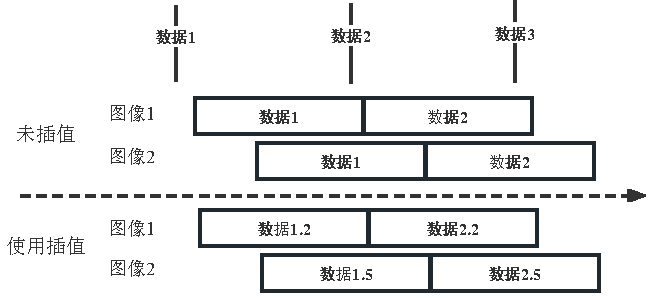
\includegraphics[width=\textwidth]{pictures/lerp.pdf}
        \caption{利用缓冲数据插值}
        \label{lerp}
    \end{center}
\end{figure}
\par
插值的一般表示方法如下方公式表示,根据起点from,终点to和一个比例t得到一个位于两者之间的位置。
在本场景中起点与终点非常明确,它们就是位于缓冲中前后两个指令中的数据。如何获得每个图像生成器的帧开始时间在两个数据中的相对位置是需要重点解决的问题。
$$Lerp(from,to,t)=from+(to-from)*t$$
\par
本系统中有一个十分重要的前提条件,仿真机产生指令数据的频率是绝对固定的。如果仿真机工作在60Hz的频率下,那么前后两次发送指令的间隔应该为16.67毫秒。
即使这些指令最终到达图像生成器的频率并不十分稳定,但是由于网络帧缓存机制的存在,依旧可以认定其时间间隔为16.67毫秒。
如果为每条指令添加一个次序信息,就可以通过频率知道它应当被处理的时刻,这个时刻对所有图像生成器都是统一的。每个图像生成器的帧开始时间是真正处理该指令的时刻,使用两个时刻的差值除以16.67毫秒后便是帧开始时间位于两个指令数据中的位置。
\par
图\ref{lerp}
\begin{figure}[h!]
    \centering
     \lstinputlisting[basicstyle= \zihao{-5}]{pictures/lerp.txt}
    \caption{网络帧缓冲机制代码}
    \label{lerpcode}
\end{figure}
\section{最终测试}
经过以上的优化后,本文对系统再次进行了测试。
本次测试中还做出了用光纤转DP的方式代替30米HDMI线连接投影仪,用3090显卡代替散热较差会产生降频的A6000显卡等变动。这些改变都能提升系统的稳定性。
\subsection{功能测试}
功能测试部分对比了本视景系统与原视景系统在相同操作下的投影图像情况。测试选择广州白云机场,分别进行了昼夜更替,天气变换,灯光控制等指令的测试,
并对比了使用同一条预设飞行路径的飞行过程。原视景系统的运行效果如图\ref{flightffs}所示,飞机即将晴朗的白天在白云机场02L号跑道上完成起飞。
图\ref{flightffs}则展示了本视景系统的运行情况,可以根据仿真机指令控制产生类似的环境效果,且后续飞行的路线与原视景系统完全一致。
目前本视景系统仍存在球幕上颜色不准确的问题,但对于数据交换子系统而言已经实现了核心功能。
\begin{figure}[h!]
    \begin{center}
        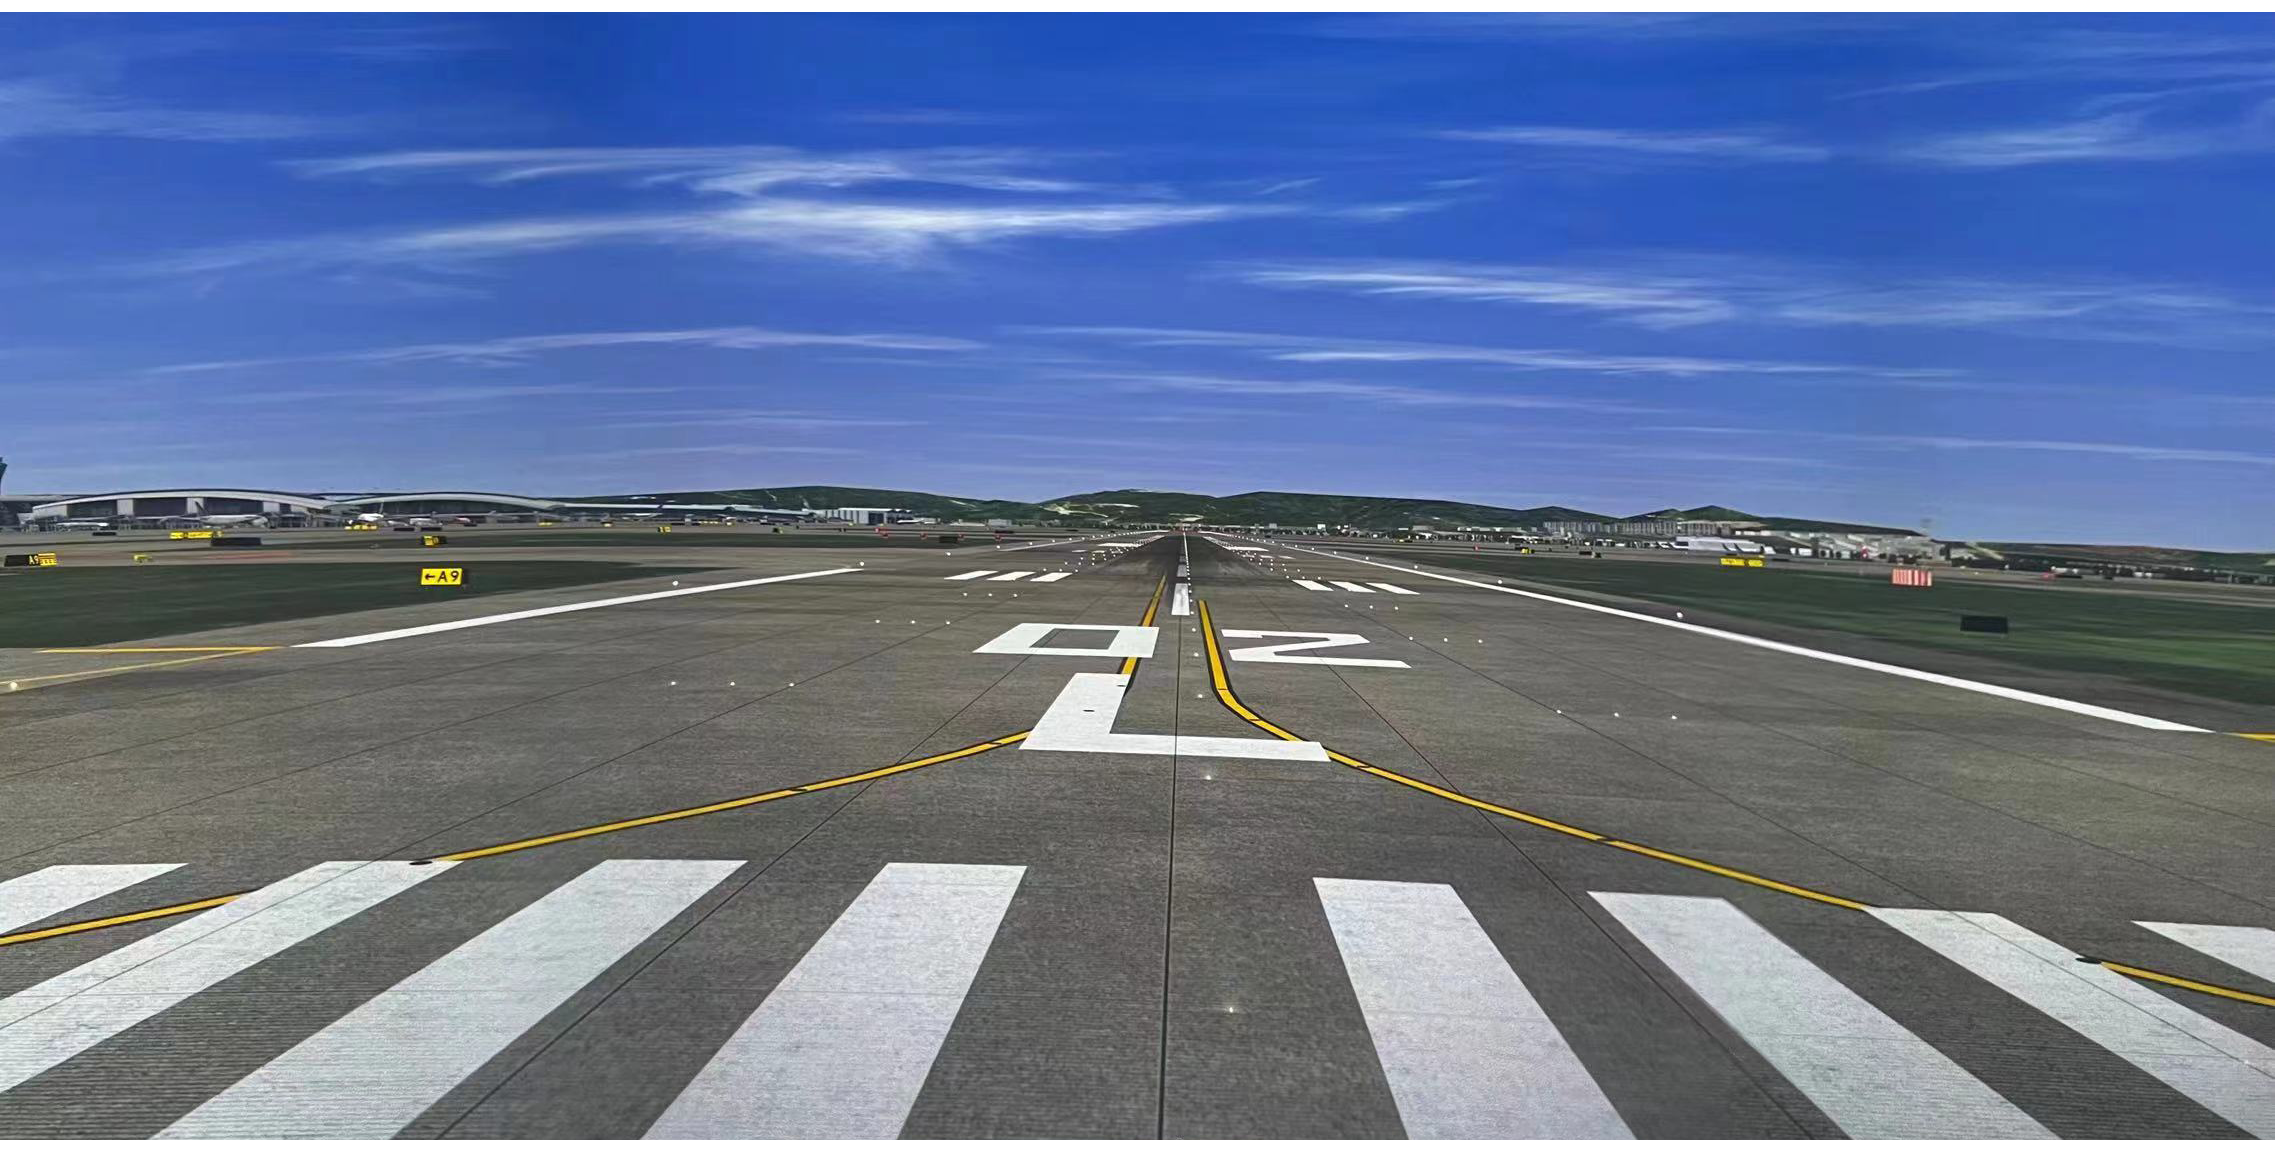
\includegraphics[width=.8\textwidth]{pictures/ffs2.png}
        \caption{原视景系统运行效果}
        \label{flightffs}
    \end{center}
\end{figure}
\begin{figure}[h!]
    \begin{center}
        \includegraphics[width=.8\textwidth]{pictures/ffs.png}
        \caption{本视景系统运行效果}
        \label{flighttest}
    \end{center}
\end{figure}
\subsection{性能测试}
性能测试的部分主要测试连续运行下视景系统的帧率稳定性。帧率检测使用第三方的监控软件,连续飞行30分钟,记录平均帧率、最高帧率、最低帧率和1\% Low帧的情况。
其中最高帧率与最低帧率并不是某一时刻的帧率,而是极短时间内的平均帧率。1\% Low是选取了帧生成时间最长的1\%的帧计算的平均帧率,这些帧不一定是连续的,所以一般会低于最低帧率,
表示整段测试时间内某些时刻的剧烈帧率波动。
\par
测试结果如表\ref{frametest}所示。本视景系统为了达成60帧率的基本要求,在数据传输、图像渲染等多方面上做出改善和取舍,根据结果也可知本视景系统在当前设备的支持下比较吃力的基本达到要求。
而原视景系统是在锁定60帧率后的运行结果,整个过程非常稳定。
1\%Low两方有非常大的差距,说明在某些复杂场景下本视景系统会产生比较剧烈的瞬时帧率波动。
\begin{table}[h!]
    \begin{center}
        \caption{帧率测试结果表}
        \label{frametest}
        \renewcommand\arraystretch{1.5}
        \begin{tabularx}{0.8\textwidth}{ 
             |>{\centering\arraybackslash\hsize=\hsize\linewidth=\hsize}X 
             |>{\centering\arraybackslash\hsize=\hsize\linewidth=\hsize}X 
             |>{\centering\arraybackslash\hsize=\hsize\linewidth=\hsize}X 
             |
             }
             \hline 
            \textbf{项目} & \textbf{本视景系统}& \textbf{原视景系统}\\   
             \hline
             运行时间 & 1802.015s & 1806.228s\\
             \hline
             总帧数 & 105418 Frame & 108735 Frame\\     
             \hline
             平均帧率 & 58.5 FPS & 60.2 FPS\\
             \hline 
             最低帧率 & 48.6 FPS & 59.2 FPS\\
             \hline 
             最高帧率 & 60.8 FPS & 60.8 FPS\\
             \hline 
             1\% Low & 38.1 FPS & 56.7 FPS\\
             \hline  
            \end{tabularx}
    \end{center}
\end{table}

\section{本章小结}
本章首先对于数据交换子系统处理已核实指令的能力做了测试,根据投影图像结果可知,该系统可以正确转换并传输双方的指令。
使用多图像生成器融合投影时先后发现图像存在撕裂和抖动的现象,经过排查分析,引入了网络帧缓冲和插值机制缓解了问题。
最终将本视景系统与原视景系统进行了对比,在功能方面两方基本一致,但帧率稳定性仍需提升。